\clearpage
\section{Source-connected local copper temperatures and gas coupling}
The original source defines three formed copper paths rather than isothermal electrical nets. Source line and arc coordinates locate 39 gas-face centroids on the contact-centered foil segments; 18 other formed-tab faces remain unresolved because their centroids do not identify a valid local segment position. The original reduced contact resistance is an assumed thermal input, not a measured interface property. With no gas heat on the foil, each constant-property segment has
\begin{equation}
T(u)=(1-u)T_0+uT_1+\frac{I^2R}{2G}u(1-u),\quad 0\leq u\leq1,
\end{equation}
where $G=kA/L$, $R$ is segment electrical resistance, and the endpoint temperatures are saved foil nodes. This solves the stated one-dimensional energy balance; it does not supply a measured or three-dimensional surface field.

The mapped foil-centroid ranges are 273.844--299.078 K for net 58, 249.439--268.080 K for net 80 and 249.783--298.380 K for net 88; maximum segment Joule curvature is below 0.030 K in this saved state. A separate analytic uniform-bath segment operator satisfies endpoint-plus-Joule energy balance and agrees with a refined independent one-dimensional numerical control. Its bath conductance is an input, not a native-cavity measurement.

\begin{figure}[htbp]
\centering
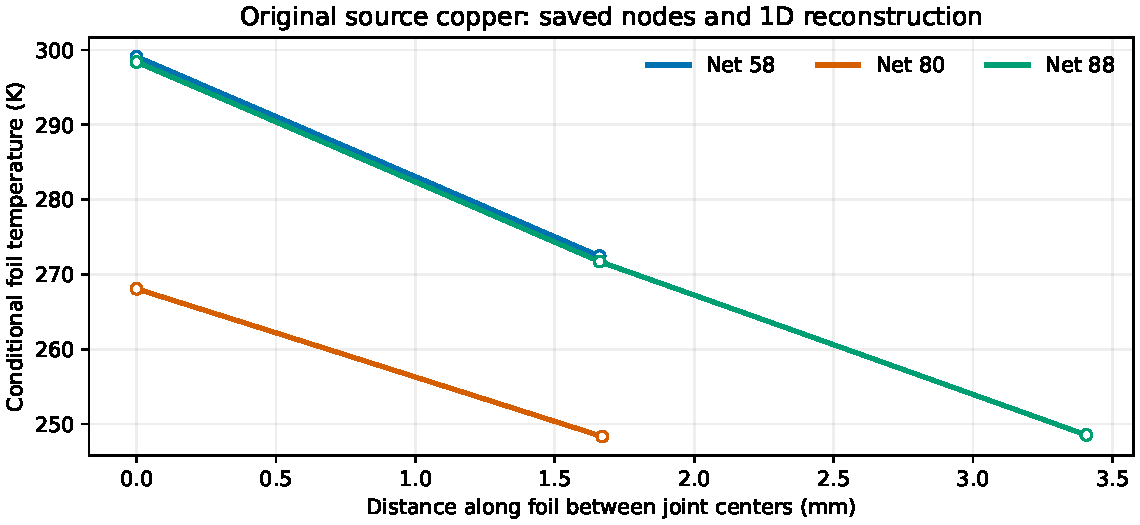
\includegraphics[width=.84\textwidth]{figures/v326_source_tab_temperature.pdf}
\caption{Saved foil contact-node temperatures and conditional one-dimensional interpolation along original source foil paths. The middle net 88 node is a thermal contact and is not an additional series electrical contact.}
\end{figure}

For illustration only, a 15 $\mu$m copper film with assumed conductivity 200--400 W/(m K) and heat flux 1000 W/m$^2$ has a through-film drop of 0.0000375--0.000075 K; unmeasured metal--ceramic contact and in-plane spreading are excluded. Of 1840 gas-facing faces, 39 have conditional distributed-tab centroid mappings, 1667 retain earlier approximate thermal proxies, and 134 remain unresolved. No additional metal--gas path is yet certified: finite paired areas, obstruction-free paths, and disjoint ownership must first be established from the actual trimmed surfaces. No new coupled temperature was solved, and the earlier electrical and gas-flux failures remain unchanged.
